%%%%%%%%%%%%%%%%%%%%%%%%%%%%%%%%%%%%%%%%%%%%%%%%%%%%%%%%%%%%%%%%%%%%%%%%%%%%%%%%%%%%%%%%%%%%%%%%%%%%%%%%%%%%%%%%%%%%%%%%%%%%%%%%%%%%%%%%%%%%%%%%%%%%%%%%%%%
% This is just an example/guide for you to refer to when submitting manuscripts to Frontiers, it is not mandatory to use Frontiers .cls files nor frontiers.tex  %
% This will only generate the Manuscript, the final article will be typeset by Frontiers after acceptance.
%                                              %
%                                                                                                                                                         %
% When submitting your files, remember to upload this *tex file, the pdf generated with it, the *bib file (if bibliography is not within the *tex) and all the figures.
%%%%%%%%%%%%%%%%%%%%%%%%%%%%%%%%%%%%%%%%%%%%%%%%%%%%%%%%%%%%%%%%%%%%%%%%%%%%%%%%%%%%%%%%%%%%%%%%%%%%%%%%%%%%%%%%%%%%%%%%%%%%%%%%%%%%%%%%%%%%%%%%%%%%%%%%%%%

%%% Version 3.4 Generated 2018/06/15 %%%
%%% You will need to have the following packages installed: datetime, fmtcount, etoolbox, fcprefix, which are normally inlcuded in WinEdt. %%%
%%% In http://www.ctan.org/ you can find the packages and how to install them, if necessary. %%%

\documentclass[utf8]{frontiersHLTH}

%\setcitestyle{square} % for Physics and Applied Mathematics and Statistics articles
\usepackage{url,hyperref,lineno,microtype,subcaption}
\usepackage[onehalfspacing]{setspace}

\linenumbers


% BELOW TAKEN FROM rticles plos template
%
% amsmath package, useful for mathematical formulas
\usepackage{amsmath}
% amssymb package, useful for mathematical symbols
\usepackage{amssymb}

% hyperref package, useful for hyperlinks
\usepackage{hyperref}

% graphicx package, useful for including eps and pdf graphics
% include graphics with the command \includegraphics
\usepackage{graphicx}

% Sweave(-like)
\usepackage{fancyvrb}
\DefineVerbatimEnvironment{Sinput}{Verbatim}{fontshape=sl}
\DefineVerbatimEnvironment{Soutput}{Verbatim}{}
\DefineVerbatimEnvironment{Scode}{Verbatim}{fontshape=sl}
\newenvironment{Schunk}{}{}
\DefineVerbatimEnvironment{Code}{Verbatim}{}
\DefineVerbatimEnvironment{CodeInput}{Verbatim}{fontshape=sl}
\DefineVerbatimEnvironment{CodeOutput}{Verbatim}{}
\newenvironment{CodeChunk}{}{}

% cite package, to clean up citations in the main text. Do not remove.
\usepackage{cite}

\usepackage{color}

\providecommand{\tightlist}{%
  \setlength{\itemsep}{0pt}\setlength{\parskip}{0pt}}

% Below is from frontiers
%
\bibliographystyle{frontiersinSCNS}
% Use doublespacing - comment out for single spacing
%\usepackage{setspace}
%\doublespacing


% Leave a blank line between paragraphs instead of using \\


\def\keyFont{\fontsize{8}{11}\helveticabold }


%% ** EDIT HERE **
%% PLEASE INCLUDE ALL MACROS BELOW

%% END MACROS SECTION



\usepackage{color}
\usepackage{fancyvrb}
\newcommand{\VerbBar}{|}
\newcommand{\VERB}{\Verb[commandchars=\\\{\}]}
\DefineVerbatimEnvironment{Highlighting}{Verbatim}{commandchars=\\\{\}}
% Add ',fontsize=\small' for more characters per line
\usepackage{framed}
\definecolor{shadecolor}{RGB}{248,248,248}
\newenvironment{Shaded}{\begin{snugshade}}{\end{snugshade}}
\newcommand{\AlertTok}[1]{\textcolor[rgb]{0.94,0.16,0.16}{#1}}
\newcommand{\AnnotationTok}[1]{\textcolor[rgb]{0.56,0.35,0.01}{\textbf{\textit{#1}}}}
\newcommand{\AttributeTok}[1]{\textcolor[rgb]{0.77,0.63,0.00}{#1}}
\newcommand{\BaseNTok}[1]{\textcolor[rgb]{0.00,0.00,0.81}{#1}}
\newcommand{\BuiltInTok}[1]{#1}
\newcommand{\CharTok}[1]{\textcolor[rgb]{0.31,0.60,0.02}{#1}}
\newcommand{\CommentTok}[1]{\textcolor[rgb]{0.56,0.35,0.01}{\textit{#1}}}
\newcommand{\CommentVarTok}[1]{\textcolor[rgb]{0.56,0.35,0.01}{\textbf{\textit{#1}}}}
\newcommand{\ConstantTok}[1]{\textcolor[rgb]{0.00,0.00,0.00}{#1}}
\newcommand{\ControlFlowTok}[1]{\textcolor[rgb]{0.13,0.29,0.53}{\textbf{#1}}}
\newcommand{\DataTypeTok}[1]{\textcolor[rgb]{0.13,0.29,0.53}{#1}}
\newcommand{\DecValTok}[1]{\textcolor[rgb]{0.00,0.00,0.81}{#1}}
\newcommand{\DocumentationTok}[1]{\textcolor[rgb]{0.56,0.35,0.01}{\textbf{\textit{#1}}}}
\newcommand{\ErrorTok}[1]{\textcolor[rgb]{0.64,0.00,0.00}{\textbf{#1}}}
\newcommand{\ExtensionTok}[1]{#1}
\newcommand{\FloatTok}[1]{\textcolor[rgb]{0.00,0.00,0.81}{#1}}
\newcommand{\FunctionTok}[1]{\textcolor[rgb]{0.00,0.00,0.00}{#1}}
\newcommand{\ImportTok}[1]{#1}
\newcommand{\InformationTok}[1]{\textcolor[rgb]{0.56,0.35,0.01}{\textbf{\textit{#1}}}}
\newcommand{\KeywordTok}[1]{\textcolor[rgb]{0.13,0.29,0.53}{\textbf{#1}}}
\newcommand{\NormalTok}[1]{#1}
\newcommand{\OperatorTok}[1]{\textcolor[rgb]{0.81,0.36,0.00}{\textbf{#1}}}
\newcommand{\OtherTok}[1]{\textcolor[rgb]{0.56,0.35,0.01}{#1}}
\newcommand{\PreprocessorTok}[1]{\textcolor[rgb]{0.56,0.35,0.01}{\textit{#1}}}
\newcommand{\RegionMarkerTok}[1]{#1}
\newcommand{\SpecialCharTok}[1]{\textcolor[rgb]{0.00,0.00,0.00}{#1}}
\newcommand{\SpecialStringTok}[1]{\textcolor[rgb]{0.31,0.60,0.02}{#1}}
\newcommand{\StringTok}[1]{\textcolor[rgb]{0.31,0.60,0.02}{#1}}
\newcommand{\VariableTok}[1]{\textcolor[rgb]{0.00,0.00,0.00}{#1}}
\newcommand{\VerbatimStringTok}[1]{\textcolor[rgb]{0.31,0.60,0.02}{#1}}
\newcommand{\WarningTok}[1]{\textcolor[rgb]{0.56,0.35,0.01}{\textbf{\textit{#1}}}}

\def\Authors{
  Dr Harry Fisher\,\textsuperscript{1*},
  Dr Marianne Gittoes\,\textsuperscript{1},
  Professor Lynne Evans\,\textsuperscript{1},
  Miss Leah Bitchell\,\textsuperscript{1},
  Dr Richard Mullen\,\textsuperscript{2},
  Dr Marco Scutari\,\textsuperscript{3}}

\def\Address{

  \textsuperscript{1} School of Sport and Health Science, Cardiff Metropolitan University,  Cardiff,   United Kingdom
  
  \textsuperscript{2} Division of Sport, Health \& Exercise Sciences, Brunel University,  London,   United Kingdom
  
  \textsuperscript{3} Istituto Dalle Molle di Studi sull'Intelligenza Artificiale (IDSIA),  Manno,   Switzerland
  }

  \def\corrAuthor{Dr Harry Fisher}\def\corrAddress{Cardiff Metropolitan University\\Cyncoed Road\\, CF23 6XD United Kingdom}\def\corrEmail{\href{mailto:harryfisher21@gmail.com}{\nolinkurl{harryfisher21@gmail.com}}}
  \def\firstAuthorLast{Fisher {et~al.}}
  
  
  
  
  
  
  
  
  
  


\begin{document}
\onecolumn
\firstpage{1}

\title[Short Title]{An interdisciplinary examination of stress and injury occurrence in
athletes}
\author[\firstAuthorLast]{\Authors}
\address{} %This field will be automatically populated
\correspondance{} %This field will be automatically populated

\extraAuth{}% If there are more than 1 corresponding author, comment this line and uncomment the next one.
%\extraAuth{corresponding Author2 \\ Laboratory X2, Institute X2, Department X2, Organization X2, Street X2, City X2 , State XX2 (only USA, Canada and Australia), Zip Code2, X2 Country X2, email2@uni2.edu}


\maketitle

\begin{abstract}

This paper adopts an interdisciplinary approach to explore the relationship between psychosocial factors, physiological stress-related markers and occurrence of injury in athletes using a repeated measures design across a 2-year data collection period. At three data collection time-points, athletes completed measures of major life events, the reinforcement sensitivity theory personality questionnaire, muscle stiffness, heart rate variability and postural stability, and reported any injuries they had sustained since the last data collection. Two Bayesian networks were used to examine the relationships between variables and model the changes between data collection points in the study. Findings revealed muscle stiffness to have the strongest relationship with injury occurrence, with high levels of stiffness increasing the probability of sustaining an injury. Negative life events did not increase the probability of injury occurrence at any single time-point; however, when examining changes between time points, increases in negative life events did increase the probability of injury. In addition, the combination of increases in negative life events and muscle stiffness resulted in the greatest probability of sustaining an injury. Findings demonstrated the importance of both an interdisciplinary approach and a repeated measures design to furthering our understanding of the relationship between stress-related  markers and injury occurrence.

\tiny
 \keyFont{ \section{Keywords:} Sports Injury, Stress, Interdisciplinary, Bayesian Network} 

\end{abstract}

\hypertarget{introduction}{%
\section*{Introduction}\label{introduction}}
\addcontentsline{toc}{section}{Introduction}

Over the last four decades sport related injuries have received
increased research attention (Ivarsson et al., 2017). This attention is
unsurprising given the high incidence (Rosa et al., 2014; Sheu et al.,
2016), and undesirable physical and psychological effects of sports
injuries (Leddy et al., 1994; Brewer, 2012). To mitigate against both
the increasing incidence and undesirable consequences of injury,
research has identified several psychological (Slimani et al., 2018),
anatomical (Murphy et al., 2003), biomechanical (Neely, 1998; Hughes,
2014) and environmental (Meeuwisse et al., 2007) factors associated with
sports injury occurrence. Indeed, several models of injury causation
have been proposed that highlight the multifactorial nature of injury
occurrence (Kumar, 2001; Meeuwisse et al., 2007; Wiese-Bjornstal, 2009),
of which one of the most widely cited was developed by Williams and
Anderson (Fig \ref{fig:fig1}; Andersen and Williams, 1988; Williams and
Andersen, 1998).

\begin{figure}[!h]
\caption{{\bf Stress and injury model (Williams and Andersen, 1998).}}
\label{fig:fig1}
\end{figure}

Williams and Andersen's (Williams and Andersen, 1998) model proposed
that when faced with a potentially stressful athletic situation, an
athlete's personality traits (e.g., hardiness, locus of control and
competitive trait anxiety), history of stressors (e.g., major life
events and previous injuries) and coping resources (e.g., general coping
behaviours) will contribute to their response, either interactively or
in isolation. Central to the model is the stress response, which
reflects the bi-directional relationship between athletes' appraisal of,
and response to, a stressful athletic situation. The model predicts that
athletes who have a history of many stressors, personality traits that
intensify the stress response and few coping resources, will exhibit
greater attentional (e.g., peripheral narrowing) and/or physiological
(e.g., increased muscle tension) responses that put these individuals at
greater risk of injury.

Within Williams and Andersen's (Williams and Andersen, 1998) model,
major life events, a component of an athlete's history of stressors,
most consistently predicts injury occurrence (Williams and Andersen,
2007); specifically, major life events with a negative, as opposed to
positive, valence (Passer and Seese, 1983; Maddison and Prapavessis,
2005). However, personality traits and coping resources have also been
found to predict injury, with for example, athletes more likely to
sustain an injury if they have poor social support and psychological
coping skills, and high trait anxiety and elevated competitive state
anxiety; compared to athletes with the opposite profile. (Smith et al.,
1990; Lavallée and Flint, 1996; Ivarsson and Johnson, 2010). However,
the amount of variance explained by the psychosocial factors proposed by
the model has been modest, typically between 5 - 30\% (Galambos et al.,
2005; Ivarsson and Johnson, 2010); suggesting other factors are also
likely to contribute to injury occurrence.

Research that has explored the effects of the psychosocial factors in
Williams and Andersen's (Williams and Andersen, 1998) model, has failed
to examine the mechanisms through which these factors are proposed to
exert their effect. To elaborate, the model suggests that injuries are
likely to occur through either increased physiological arousal resulting
in increased muscle tension and reduced flexibility or attentional
deficits caused by increased distractibility and peripheral narrowing.
However, to date, the research has largely focused on attentional
deficits (Andersen and Williams, 1999; Rogers and Landers, 2005;
Wilkerson, 2012; Swanik et al., 2007). For example, Andersen and
Williams (Andersen and Williams, 1999) measured peripheral and central
vision during high and low stress conditions and found athletes with
high life event stress coupled with low social support had greater
peripheral narrowing under stressful conditions compared to athletes
with the opposing profile; these athletes went on to sustain an
increased number of injuries during the following season. Indeed,
Rodgers and Landers (Rogers and Landers, 2005) supported Andersen and
Williams's (Andersen and Williams, 1999) earlier findings reporting that
peripheral narrowing under stress mediated 8.1\% of the relationship
between negative life events and injury. However, few attempts have been
made to explain the remaining variance between negative life events and
athletic injury through the other proposed mechanisms, such as increased
muscle tension and reduced motor control (cf.~Williams and Andersen,
1998).

One possible reason for this oversight is the multifactorial nature of
injury and the possible contribution of other non-psychological factors
to the stress response (Meeuwisse et al., 2007; Wiese-Bjornstal, 2009).
For example, a large body of research indicates that training-related
stress is also likely to be related to the stress response and injury
occurrence (Lee et al., 2017; Djaoui et al., 2017), and may account for
the unexplained variance from the psychological predictors of injury.
Appaneal and Perna (Appaneal and Perna, 2014) proposed the
biopsychosocial model of stress athletic injury and health (BMSAIH) to
serve as an extension to Williams and Andersen's (Williams and Andersen,
1998) model and to address some of these issues. To elaborate, the
BMSAIH aimed to clarify the mediating pathways between the stress
response and injury, consider other health outcomes and behavioural
factors that impact sports participation, and integrate the impact of
training on athletes' health (Appaneal and Perna, 2014). The central
tenet of the BMSAIH is that psychosocial distress (e.g., negative life
events) may act synergistically with training-related stress as a result
of high-intensity and high-volume sports training, and ``widen the
window of susceptibility'' (Appaneal and Perna, 2014, 74) to a range of
undesirable health outcomes including illness and injury. Consequently,
the BMSAIH provides a framework for future research to build on Williams
and Andersen's (Williams and Andersen, 1998) model, by including other
physiological markers of training-related stress, which together may
provide greater insight into the injury process.

Although research supporting the BMSAIH has mainly focused on the
relationship between hormonal responses to training and injury
occurrence (Perna and McDowell, 1995; Perna et al., 1997, 2003), other
research has identified additional markers of training-related stress
that are associated with an increased risk of injury; for example, heart
rate variability (Bellenger et al., 2016; Williams et al., 2017),
postural stability (Romero-Franco et al., 2014) and muscle stiffness
(Pruyn et al., 2015). Unfortunately, these markers are often studied in
isolation without an assessment of the psychosocial factors that are
known to contribute to injury, thereby limiting our understanding of how
psychosocially and physiologically derived stress may contribute
synergistically to injury occurrence. Recently, Bittencourt et
al.~(Bittencourt et al., 2016) suggested that to better understand the
multifactorial nature of sports injuries, research needs to move away
from studying risk factors in isolation and instead adopt a complex
systems approach to injury. Such an approach posits that injury may
arise from a complex ``web of determinants'' (Bittencourt et al., 2016,
3), where different factors interact in unpredictable and unplanned
ways, but result in a global outcome pattern of either adaptation or
injury. Complex systems approaches have been used in health care to
model the large number of risk factors associated with different types
of diseases (Plsek and Greenhalgh, 2001); however, very few studies have
attempted to address sport injury occurrence using such an approach
(Hulme et al., 2018).

To summarise, despite offering a possible framework to build on the
research stemming from Williams and Andersen's (Williams and Andersen,
1998) model, researchers have largely overlooked the potential to
explore other physiological stress-related markers proposed by the
BMSAIH, in addition to the already well-established psychological
characteristics known to be related to injury (Appaneal and Perna,
2014). Furthermore, research has typically not captured changes in both
psychosocial factors and stress-related physiological markers that may
occur between initial measurement and injury occurrence. Viewed through
the lens of a complex systems approach the interaction between
psychosocial sources of stress, stress-related physiological markers and
injury occurrence may provide new insight into the injury process.
Therefore, the purpose of the current study was to examine the
relationship between psychosocial factors, physiological stress-related
markers and occurrence of injury in athletes over time.

\hypertarget{results}{%
\section*{Results}\label{results}}
\addcontentsline{toc}{section}{Results}

\hypertarget{subsection-1}{%
\subsection*{Subsection 1}\label{subsection-1}}
\addcontentsline{toc}{subsection}{Subsection 1}

You can use \texttt{R} chunks directly to plot graphs.

\begin{Shaded}
\begin{Highlighting}[]
\NormalTok{x <-}\StringTok{ }\DecValTok{0}\OperatorTok{:}\DecValTok{100}
\KeywordTok{set.seed}\NormalTok{(}\DecValTok{999}\NormalTok{)}
\NormalTok{y <-}\StringTok{ }\DecValTok{2} \OperatorTok{*}\StringTok{ }\NormalTok{(x }\OperatorTok{+}\StringTok{ }\KeywordTok{rnorm}\NormalTok{(}\KeywordTok{length}\NormalTok{(x), }\DataTypeTok{sd =} \DecValTok{3}\NormalTok{) }\OperatorTok{+}\StringTok{ }\DecValTok{3}\NormalTok{)}
\KeywordTok{plot}\NormalTok{(x, y)}
\end{Highlighting}
\end{Shaded}

\hypertarget{subsection-2}{%
\subsection*{Subsection 2}\label{subsection-2}}
\addcontentsline{toc}{subsection}{Subsection 2}

Frontiers requires figures to be submitted individually, in the same
order as they are referred to in the manuscript. Figures will then be
automatically embedded at the bottom of the submitted manuscript. Kindly
ensure that each table and figure is mentioned in the text and in
numerical order. Permission must be obtained for use of copyrighted
material from other sources (including the web). Please note that it is
compulsory to follow figure instructions. Figures which are not
according to the guidelines will cause substantial delay during the
production process.

\hypertarget{discussion}{%
\section{Discussion}\label{discussion}}

\hypertarget{disclosureconflict-of-interest-statement}{%
\section*{Disclosure/Conflict-of-Interest
Statement}\label{disclosureconflict-of-interest-statement}}
\addcontentsline{toc}{section}{Disclosure/Conflict-of-Interest
Statement}

The authors declare that the research was conducted in the absence of
any commercial or financial relationships that could be construed as a
potential conflict of interest.

\hypertarget{author-contributions}{%
\section*{Author Contributions}\label{author-contributions}}
\addcontentsline{toc}{section}{Author Contributions}

The statement about the authors and contributors can be up to several
sentences long, describing the tasks of individual authors referred to
by their initials and should be included at the end of the manuscript
before the References section.

\hypertarget{acknowledgments}{%
\section*{Acknowledgments}\label{acknowledgments}}
\addcontentsline{toc}{section}{Acknowledgments}

Funding:

\hypertarget{supplemental-data}{%
\section{Supplemental Data}\label{supplemental-data}}

Supplementary Material should be uploaded separately on submission, if
there are Supplementary Figures, please include the caption in the same
file as the figure. LaTeX Supplementary Material templates can be found
in the Frontiers LaTeX folder

\hypertarget{references}{%
\section{References}\label{references}}

A reference list should be automatically created here. However it won't.
Pandoc will place the list of references at the end of the document
instead. There are no convenient solution for now to force Pandoc to do
otherwise. The easiest way to get around this problem is to edit the
LaTeX file created by Pandoc before compiling it again using the
traditional LaTeX commands.

\hypertarget{figures}{%
\section*{Figures}\label{figures}}
\addcontentsline{toc}{section}{Figures}

\begin{figure}

{\centering 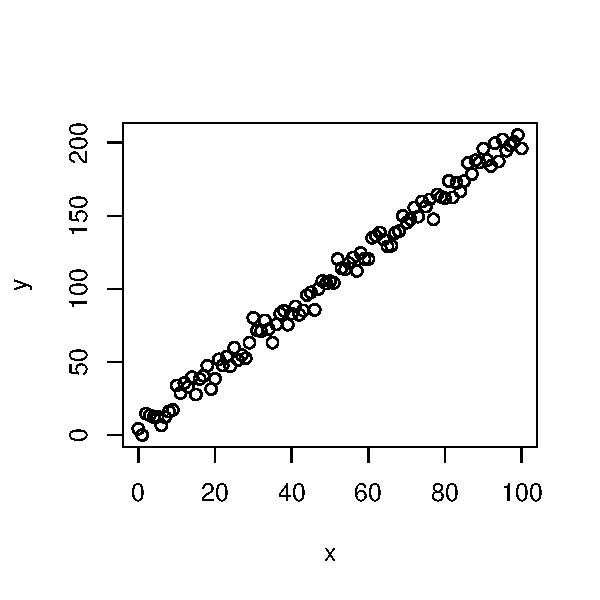
\includegraphics[width=85mm,height=85mm]{full_paper_v2_files/figure-latex/Figure-1-1} 

}

\caption{Figure caption}\label{fig:Figure-1}
\end{figure}

\hypertarget{refs}{}
\leavevmode\hypertarget{ref-Andersen1988}{}%
Andersen, M. B., and Williams, J. M. (1988). A model of stress and
athletic injury: Prediction and prevention. \emph{Journal of Sport and
Exercise Psychology} 10, 294--306.
doi:\href{https://doi.org/10.1123/jsep.10.3.294}{10.1123/jsep.10.3.294}.

\leavevmode\hypertarget{ref-Andersen1999}{}%
Andersen, M. B., and Williams, J. M. (1999). Athletic injury,
psychosocial factors and perceptual changes during stress. \emph{Journal
of Sports Sciences} 17, 735--741.
doi:\href{https://doi.org/10.1080/026404199365597}{10.1080/026404199365597}.

\leavevmode\hypertarget{ref-Appaneal2014}{}%
Appaneal, R. N., and Perna, F. M. (2014). ``Biopsychosocial model of
injury,'' in \emph{Encyclopedia of sport and exercise psychology}, eds.
R. C. Eklund and G. Tenenbaum (Thousand Oaks, CA: Sage), 74--77.

\leavevmode\hypertarget{ref-Bellenger2016}{}%
Bellenger, C. R., Fuller, J. T., Thomson, R. L., Davison, K., Robertson,
E. Y., and Buckley, J. D. (2016). Monitoring athletic training status
through autonomic heart rate regulation: A systematic review and
meta-analysis. \emph{Sports Medicine} 46, 1461--1486.
doi:\href{https://doi.org/10.1007/s40279-016-0484-2}{10.1007/s40279-016-0484-2}.

\leavevmode\hypertarget{ref-Bittencourt2016}{}%
Bittencourt, N. F. N., Meeuwisse, W. H., Mendonça, L. D.,
Nettel-Aguirre, A., Ocarino, J. M., and Fonseca, S. T. (2016). Complex
systems approach for sports injuries: Moving from risk factor
identification to injury pattern recognition - narrative review and new
concept. \emph{British Journal of Sports Medicine} 50, 1309--1314.
doi:\href{https://doi.org/10.1136/bjsports-2015-095850}{10.1136/bjsports-2015-095850}.

\leavevmode\hypertarget{ref-Brewer2012}{}%
Brewer, B. W. (2012). ``Psychology of sport injury rehabilitation,'' in
\emph{Handbook of sport psychology}, eds. G. Tenenbaum and R. C. Eklund
(Hoboken, NJ, USA: Wiley), 404--424.
doi:\href{https://doi.org/10.1002/9781118270011.ch18}{10.1002/9781118270011.ch18}.

\leavevmode\hypertarget{ref-Djaoui2017}{}%
Djaoui, L., Haddad, M., Chamari, K., and Dellal, A. (2017). Monitoring
training load and fatigue in soccer players with physiological markers.
\emph{Physiology and Behavior} 181, 86--94.
doi:\href{https://doi.org/10.1016/j.physbeh.2017.09.004}{10.1016/j.physbeh.2017.09.004}.

\leavevmode\hypertarget{ref-Galambos2005}{}%
Galambos, S. A., Terry, P. C., Moyle, G. M., and Locke, S. A. (2005).
Psychological predictors of injury among elite athletes. \emph{British
Journal of Sports Medicine} 39, 351--354.
doi:\href{https://doi.org/10.1136/bjsm.2005.018440}{10.1136/bjsm.2005.018440}.

\leavevmode\hypertarget{ref-Hughes2014}{}%
Hughes, G. (2014). A review of recent perspectives on biomechanical risk
factors associated with anterior cruciate ligament injury.
\emph{Research in Sports Medicine} 22, 193--212.
doi:\href{https://doi.org/10.1080/15438627.2014.881821}{10.1080/15438627.2014.881821}.

\leavevmode\hypertarget{ref-Hulme2018}{}%
Hulme, A., Thompson, J., Nielsen, R. O., Read, G. J. M. M., and Salmon,
P. M. (2018). Towards a complex systems approach in sports injury
research: Simulating running-related injury development with agent-based
modelling. \emph{British Journal of Sports Medicine} 53, 560--569.
doi:\href{https://doi.org/10.1136/bjsports-2017-098871}{10.1136/bjsports-2017-098871}.

\leavevmode\hypertarget{ref-Ivarsson2010}{}%
Ivarsson, A., and Johnson, U. (2010). Psychological factors as
predictors of injuries among senior soccer players. A prospective study.
\emph{Journal of Sports Science and Medicine} 9, 347--352. Available at:
\url{https://www.ncbi.nlm.nih.gov/pmc/articles/PMC3761721/}.

\leavevmode\hypertarget{ref-Ivarsson2017}{}%
Ivarsson, A., Johnson, U., Andersen, M. B., Tranaeus, U., Stenling, A.,
and Lindwall, M. (2017). Psychosocial factors and sport injuries:
Meta-analyses for prediction and prevention. \emph{Sports Medicine} 47,
353--365.
doi:\href{https://doi.org/10.1007/s40279-016-0578-x}{10.1007/s40279-016-0578-x}.

\leavevmode\hypertarget{ref-Kumar2001}{}%
Kumar, S. (2001). Theories of musculoskeletal injury causation.
\emph{Ergonomics} 44, 17--47.
doi:\href{https://doi.org/10.1080/00140130120716}{10.1080/00140130120716}.

\leavevmode\hypertarget{ref-Lavallee1996}{}%
Lavallée, L., and Flint, F. (1996). The relationship of stress,
competitive anxiety, mood state, and social support to athletic injury.
\emph{Journal of Athletic Training} 31, 296--299. Available at:
\url{http://www.ncbi.nlm.nih.gov/pubmed/16558413}.

\leavevmode\hypertarget{ref-Leddy1994}{}%
Leddy, M. H., Lambert, M. J., and Ogles, B. M. (1994). Psychological
consequences of athletic injury among high-level competitors.
\emph{Research Quarterly for Exercise and Sport} 65, 347--354.
doi:\href{https://doi.org/10.1080/02701367.1994.10607639}{10.1080/02701367.1994.10607639}.

\leavevmode\hypertarget{ref-Lee2017}{}%
Lee, E. C., Fragala, M. S., Kavouras, S. A., Queen, R. M., Pryor, J. L.,
and Casa, D. J. (2017). Biomarkers in sports and exercise: Tracking
health, performance, and recovery in athletes. \emph{Journal of Strength
and Conditioning Research} 31, 2920--2937.
doi:\href{https://doi.org/10.1519/JSC.0000000000002122}{10.1519/JSC.0000000000002122}.

\leavevmode\hypertarget{ref-Maddison2005}{}%
Maddison, R., and Prapavessis, H. (2005). A psychological approach to
the prediction and prevention of athletic injury. \emph{Journal of Sport
and Exercise Psychology} 27, 289--310.
doi:\href{https://doi.org/10.1123/jsep.27.3.289}{10.1123/jsep.27.3.289}.

\leavevmode\hypertarget{ref-Meeuwisse2007}{}%
Meeuwisse, W. H., Tyreman, H., Hagel, B., and Emery, C. (2007). A
dynamic model of etiology in sport injury: The recursive nature of risk
and causation. \emph{Clinical Journal of Sport Medicine} 17, 215--219.
doi:\href{https://doi.org/10.1097/JSM.0b013e3180592a48}{10.1097/JSM.0b013e3180592a48}.

\leavevmode\hypertarget{ref-Murphy2003}{}%
Murphy, D. F., Connolly, D. A. J., and Beynnon, B. D. (2003). Risk
factors for lower extremity injury: A review of the literature.
\emph{British Journal of Sports Medicine} 37, 13--29.
doi:\href{https://doi.org/10.1136/bjsm.37.1.13}{10.1136/bjsm.37.1.13}.

\leavevmode\hypertarget{ref-Neely1998}{}%
Neely, F. G. (1998). Biomechanical risk factors for exercise-related
lower limb injuries. \emph{Sports Medicine} 26, 395--413.
doi:\href{https://doi.org/10.2165/00007256-199826060-00003}{10.2165/00007256-199826060-00003}.

\leavevmode\hypertarget{ref-Passer1983a}{}%
Passer, M. W., and Seese, M. D. (1983). Life stress and athletic injury:
Examination of positive versus negative events and three moderator
variables. \emph{Journal of Human Stress} 9, 11--16.
doi:\href{https://doi.org/10.1080/0097840X.1983.9935025}{10.1080/0097840X.1983.9935025}.

\leavevmode\hypertarget{ref-Perna2003}{}%
Perna, F. M., Antoni, M. H., Baum, A., Gordon, P., and Schneiderman, N.
(2003). Cognitive behavioral stress management effects on injury and
illness among competitive athletes: A randomized clinical trial.
\emph{Annals of Behavioral Medicine} 25, 66--73. Available at:
\url{https://www.scopus.com/inward/record.uri?eid=2-s2.0-0037262738\%7B/\&\%7DpartnerID=40\%7B/\&\%7Dmd5=37332ebe6a962abf5178e51d6ebaedb7}.

\leavevmode\hypertarget{ref-Perna1995}{}%
Perna, F. M., and McDowell, S. L. (1995). Role of psychological stress
in cortisol recovery from exhaustive exercise among elite athletes.
\emph{International Journal of Behavioral Medicine} 2, 13--26.
doi:\href{https://doi.org/10.1207/s15327558ijbm0201_2}{10.1207/s15327558ijbm0201\_2}.

\leavevmode\hypertarget{ref-Perna1997}{}%
Perna, F., Schneiderman, N., and LaPerriere, A. (1997). Psychological
stress, exercise and immunity. \emph{International Journal of Sports
Medicine} 18, 78--83.
doi:\href{https://doi.org/10.1055/s-2007-972703}{10.1055/s-2007-972703}.

\leavevmode\hypertarget{ref-Plsek2001}{}%
Plsek, P. E., and Greenhalgh, T. (2001). The challenge of complexity in
health care. \emph{BMJ} 323, 625--628.
doi:\href{https://doi.org/10.1136/bmj.323.7313.625}{10.1136/bmj.323.7313.625}.

\leavevmode\hypertarget{ref-Pruyn2015}{}%
Pruyn, E. C., Watsford, M. L., and Murphy, A. J. (2015). Differences in
lower-body stiffness between levels of netball competition.
\emph{Journal of Strength and Conditioning Research} 29, 1197--1202.
doi:\href{https://doi.org/10.1519/JSC.0000000000000418}{10.1519/JSC.0000000000000418}.

\leavevmode\hypertarget{ref-Rogers2005}{}%
Rogers, T., and Landers, D. M. (2005). Mediating effects of peripheral
vision in the life event stress/athletic injury relationship.
\emph{Journal of Sport and Exercise Psychology} 27, 271--288.
doi:\href{https://doi.org/10.1002/9781444303650}{10.1002/9781444303650}.

\leavevmode\hypertarget{ref-Romero-Franco2014}{}%
Romero-Franco, N., Gallego-Izquierdo, T., Martínez-López, E. J.,
Hita-Contreras, F., Osuna-Pére, Catalina, M., and Martínez-Amat, A.
(2014). Postural stability and subsequent sports injuries during indoor
season of athletes. \emph{Journal of Physical Therapy Science} 26,
683--687.
doi:\href{https://doi.org/10.1589/jpts.26.683}{10.1589/jpts.26.683}.

\leavevmode\hypertarget{ref-Rosa2014}{}%
Rosa, B. B., Asperti, A. M., Helito, C. P., Demange, M. K., Fernandes,
T. L., and Hernandez, A. J. (2014). Epidemiology of sports injuries on
collegiate athletes at a single center. \emph{Acta Ortopédica
Brasileira} 22, 321--324.
doi:\href{https://doi.org/10.1590/1413-78522014220601007}{10.1590/1413-78522014220601007}.

\leavevmode\hypertarget{ref-Sheu2016}{}%
Sheu, Y., Chen, L. H., and Hedegaard, H. (2016). Sports- and
Recreation-related Injury Episodes in the United States, 2011-2014.
\emph{National Health Statistics Reports}, 1--12. Available at:
\url{https://www.ncbi.nlm.nih.gov/pubmed/27906643}.

\leavevmode\hypertarget{ref-Slimani2018}{}%
Slimani, M., Bragazzi, N. L., Znazen, H., Paravlic, A., Azaiez, F., and
Tod, D. (2018). Psychosocial predictors and psychological prevention of
soccer injuries: A systematic review and meta-analysis of the
literature. \emph{Physical Therapy in Sport} 32, 293--300.
doi:\href{https://doi.org/10.1016/j.ptsp.2018.05.006}{10.1016/j.ptsp.2018.05.006}.

\leavevmode\hypertarget{ref-Smith1990}{}%
Smith, R. E., Smoll, F. L., and Ptacek, J. T. (1990). Conjunctive
moderator variables in vulnerability and resiliency research: Life
stress, social support and coping skills, and adolescent sport injuries.
\emph{Journal of Personality and Social Psychology} 58, 360--370.
doi:\href{https://doi.org/10.1037/0022-3514.58.2.360}{10.1037/0022-3514.58.2.360}.

\leavevmode\hypertarget{ref-Swanik2007}{}%
Swanik, C. B., Covassin, T., Stearne, D. J., and Schatz, P. (2007). The
relationship between neurocognitive function and noncontact anterior
cruciate ligament injuries. \emph{American Journal of Sports Medicine}
35, 943--948.
doi:\href{https://doi.org/10.1177/0363546507299532}{10.1177/0363546507299532}.

\leavevmode\hypertarget{ref-Wiese-Bjornstal2009}{}%
Wiese-Bjornstal, D. M. (2009). Sport injury and college athlete health
across the lifespan. \emph{Journal of Intercollegiate Sport} 2, 64--80.
doi:\href{https://doi.org/10.1123/jis.2.1.64}{10.1123/jis.2.1.64}.

\leavevmode\hypertarget{ref-Wilkerson2012a}{}%
Wilkerson, G. B. (2012). Neurocognitive reaction time predicts lower
extremity sprains and strains. \emph{International Journal of Athletic
Therapy and Training} 17, 4--9.
doi:\href{https://doi.org/10.1123/ijatt.17.6.4}{10.1123/ijatt.17.6.4}.

\leavevmode\hypertarget{ref-Williams2007}{}%
Williams, J. M., and Andersen, M. B. (2007). ``Psychosocial antecedents
of sport injury and interventions for risk reduction,'' in
\emph{Handbook of sport psychology}, eds. G. Tenenbaum and R. C. Eklund
(Hoboken, NJ, USA: Wiley), 379--403.
doi:\href{https://doi.org/10.1002/9781118270011.ch17}{10.1002/9781118270011.ch17}.

\leavevmode\hypertarget{ref-Williams1998}{}%
Williams, J. M., and Andersen, M. B. (1998). Psychosocial antecedents of
sport injury: review and critique of the stress and injury model.
\emph{Journal of Applied Sport Psychology} 10, 5--25.
doi:\href{https://doi.org/10.1080/10413209808406375}{10.1080/10413209808406375}.

\leavevmode\hypertarget{ref-Williams2017}{}%
Williams, S., Booton, T., Watson, M., Rowland, D., and Altini, M.
(2017). Heart rate variability is a moderating factor in the
workload-injury relationship of competitive crossfit™ athletes.
\emph{Journal of Sports Science and Medicine} 16, 443--449.

\end{document}
